\section{Sentiment Analysis}
\label{chap:sent}
As stated in \citep{Veselovska}: "Sentiment analysis, also known as opinion mining, is an automatic detection of a positive or negative polarity, or neutrality of ... a text sequence", which is exactly as the sentiment analysis is understood in this work, although there are some other definitions consisting of e.g. opinion extraction, irony or stance \citep{Montoyo2012}. Another tasks related to sentiment analysis is a subjectivity analysis (whether the presented opinion is objective or highly subjective), which is also not included in this work, mainly because the lack of labelled data for Czech. It is possible to analyze individual expressions, sentences or whole documents \citep{Veselovska} and this work focuses on the document level classification.
\subsection{Task definition}
\paragraph{Sentiment analysis} \mbox{}\\
\textit{input:} sequence of sentences (a whole post or comment, depending on the source) \\
\textit{output:} prevailing sentiment of the input from categories: neutral, positive, negative.
\par

\paragraph{Metric} For evaluating performance, two metrics are used: macro-averaged F1 score and accuracy. Both metrics are chosen for better comparability with previous work.

\subsection{Related Work}
citace:
\citep{Cano2019}
\citep{Kittask2020} .. estonian

\citep{Hercig2018}
\citep{Li}

%TODO habernal vytvoril ty datasty 

%TODO celkova tabulka
There is not so many attempts to sentiment analysis in Czech in comparison to english, however some attempts were made with both neural networks and traditional machine learning - naive bayes classifiers,support vector machines, and maximum-entropy-based classifiers \citep{Veselovska}.  %TODO citace SVM Ptáček(2013), 
For a practical use \citep{Zizka} presented automatic sentiment prediction of unlabelled text based on a small set of labelled patterns via searching similarities.  One of first attepts to apply neural networks on Czech sentiment is described in \citep{Lenc}, which evaluates besides others all three datasets used in this work on document-level sentiment analysis. 

As the neural networks dominates in many NLP taks, they are also applied in sentiment analysis. \citep{kysely} performes sentiment analysis using embeddings and convolutional neural network on multidimensional embedding, which is quite unusual as CNNs are typically used for image processing. \citep{kysely} uses same three datasets, but classifies only on sentiment-level (they filtered out longer samples), which is simpler as longer texts tend to be more inconsistent about sentiment \citep{Veselovska}. \citep{Libovicky} presents state-of-the art results in three czech NLP tasks including sentiment analysis. They use only CSFD dataset with resulting accuracy 80.8\% which is comparable to previous \acrshort{sota} \citep{Brychcin2013}. The second mentioned paper uses quite complicated method for classification incorporating the fact of which movie is reviewed, while \citep{Libovicky} uses only bidirectional LSTMs with multiple attention heads following state-of-the-art results on English \citep{Lin2017}. There are four previous works know to me, which involves BERT-like models: 
\begin{itemize}
\item XLM-Roberta applied on all three datastets trimmed to 128 characters \footnote{http://www.janpalasek.com/sentiment-analysis-czech.html}
\item \citep{Klouda} applies multilingual BERT on mall dataset with resulting accuracy about  81\%, which did not outperform the naive bayes classifier baseline with 84\% accuracy, 
\item  \citep{Sido2021} presents monolingual Czech model Czert,  based on BERT and ALBERT models, and evalutes it on csfd and facebook datastets with new state-of-the-art results,
\item \citep{Straka2021} published another monolingual model, this time based on more succesfull RoBERTa model and surpassed Czert on facebook dataset.


\end{itemize}


%%%%%%%BERTI


robeczech

\subsection{Dataset and Preprocessing}
%TODO zjistit jaka jsou na to porovnavaci data This work primary tries to improve existing tasks and show the ability of contextualized embeddings to improve results, so tasks with existing data and results were selected.  %TODO why?
Four main Czech datasets with sentiment annotation are available: user reviews from MALL.cz (mall), film reviews from csfd.cz (csfd), news from Aktualne.cz (aktualne) and posts from Czech branch pages on facebook.cz (facebook). As \textit{aktualne} dataset turned out to be problematical because the text were ambiguous even for annotators, and its authors later used other mentioned datasets \citep{Veselovska}, this work also focuses only on the three other data sources -- \textit{mall}, \textit{csfd} and \textit{facebook} \footnote{All three datasets are all available here: http://liks.fav.zcu.cz/sentiment/}. Some experiment are also performed with in-domain training on Eglish data. For this purpose is used \textit{imdb} dataset \footnote{https://www.tensorflow.org/datasets/catalog/imdb\_reviews}, which contains movie review from the biggest movie rating website imdb.com. This leads to some problems described later in this section, because English dataset contains only binary classification (positive/negative). Table \ref{tab:datasets} summarize each dataset. All dataset were randomly split into train, development and test datasets with the same labels distribution as original datasets.
\par
As can be seen in figure \ref{pic:dist}, distribution of labels differs among datasets. Moreover, Figure \ref{pic:dist_all}
\begin{figure}[!h]
\centering
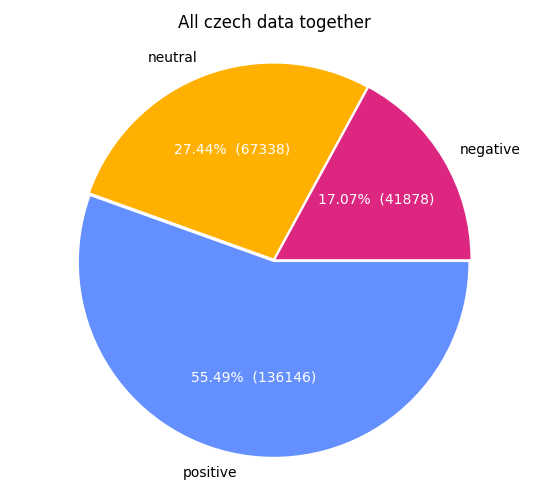
\includegraphics[width=0.7\columnwidth]{../img/all.png}
\protect\caption{Percentage and absolute values of labels in all three Czech datasets together.}
\label{pic:dist_all}
\end{figure}
%TODO all má blbý nadpis
shows, that the resulting dataset is highly unbalanced, which may causes divergence and stuck in training. Due to the big part of labels being positive, many learning strategies just ended with predicting only \textit{positive} class, i.e. 55\% accuracy, so unfortunately learned nothing. 
%TODO popis tabulky
\begin{center}
\begin{table}[]
\begin{tabular}{|l||lll|}
\hline
     & length & labels                                                                & domain        \\ \hline \hline
\textbf{mall}     & 145306 & \begin{tabular}[c]{@{}l@{}}positive\\ neutral\\ negative\end{tabular} & domestic appliance reviews                             \\ \hline
\textbf{csfd} & 91304  & \begin{tabular}[c]{@{}l@{}}positive\\ neutral\\ negative\end{tabular} & movie reviews \\ \hline
\textbf{facebook} & 9752   & \begin{tabular}[c]{@{}l@{}}positive\\ neutral\\ negative\end{tabular} & \begin{tabular}[c]{@{}l@{}}brand pages of e.g. shops or mobile network\\ providers\end{tabular} \\ \hline
\textbf{imdb} & 25000  & \begin{tabular}[c]{@{}l@{}}positive\\ negative\end{tabular}           & movie reviews \\ \hline
\end{tabular}
\caption{Three Czech datasets (mall, facebook, csfd) and one English (imdb) are used for training in this work.}
\label{tab:datasets}
\end{table}
\end{center}


%TODO je to rozdleeno se stratifikací?
%TODO popis obrazku
\begin{figure}[!h]
\centering
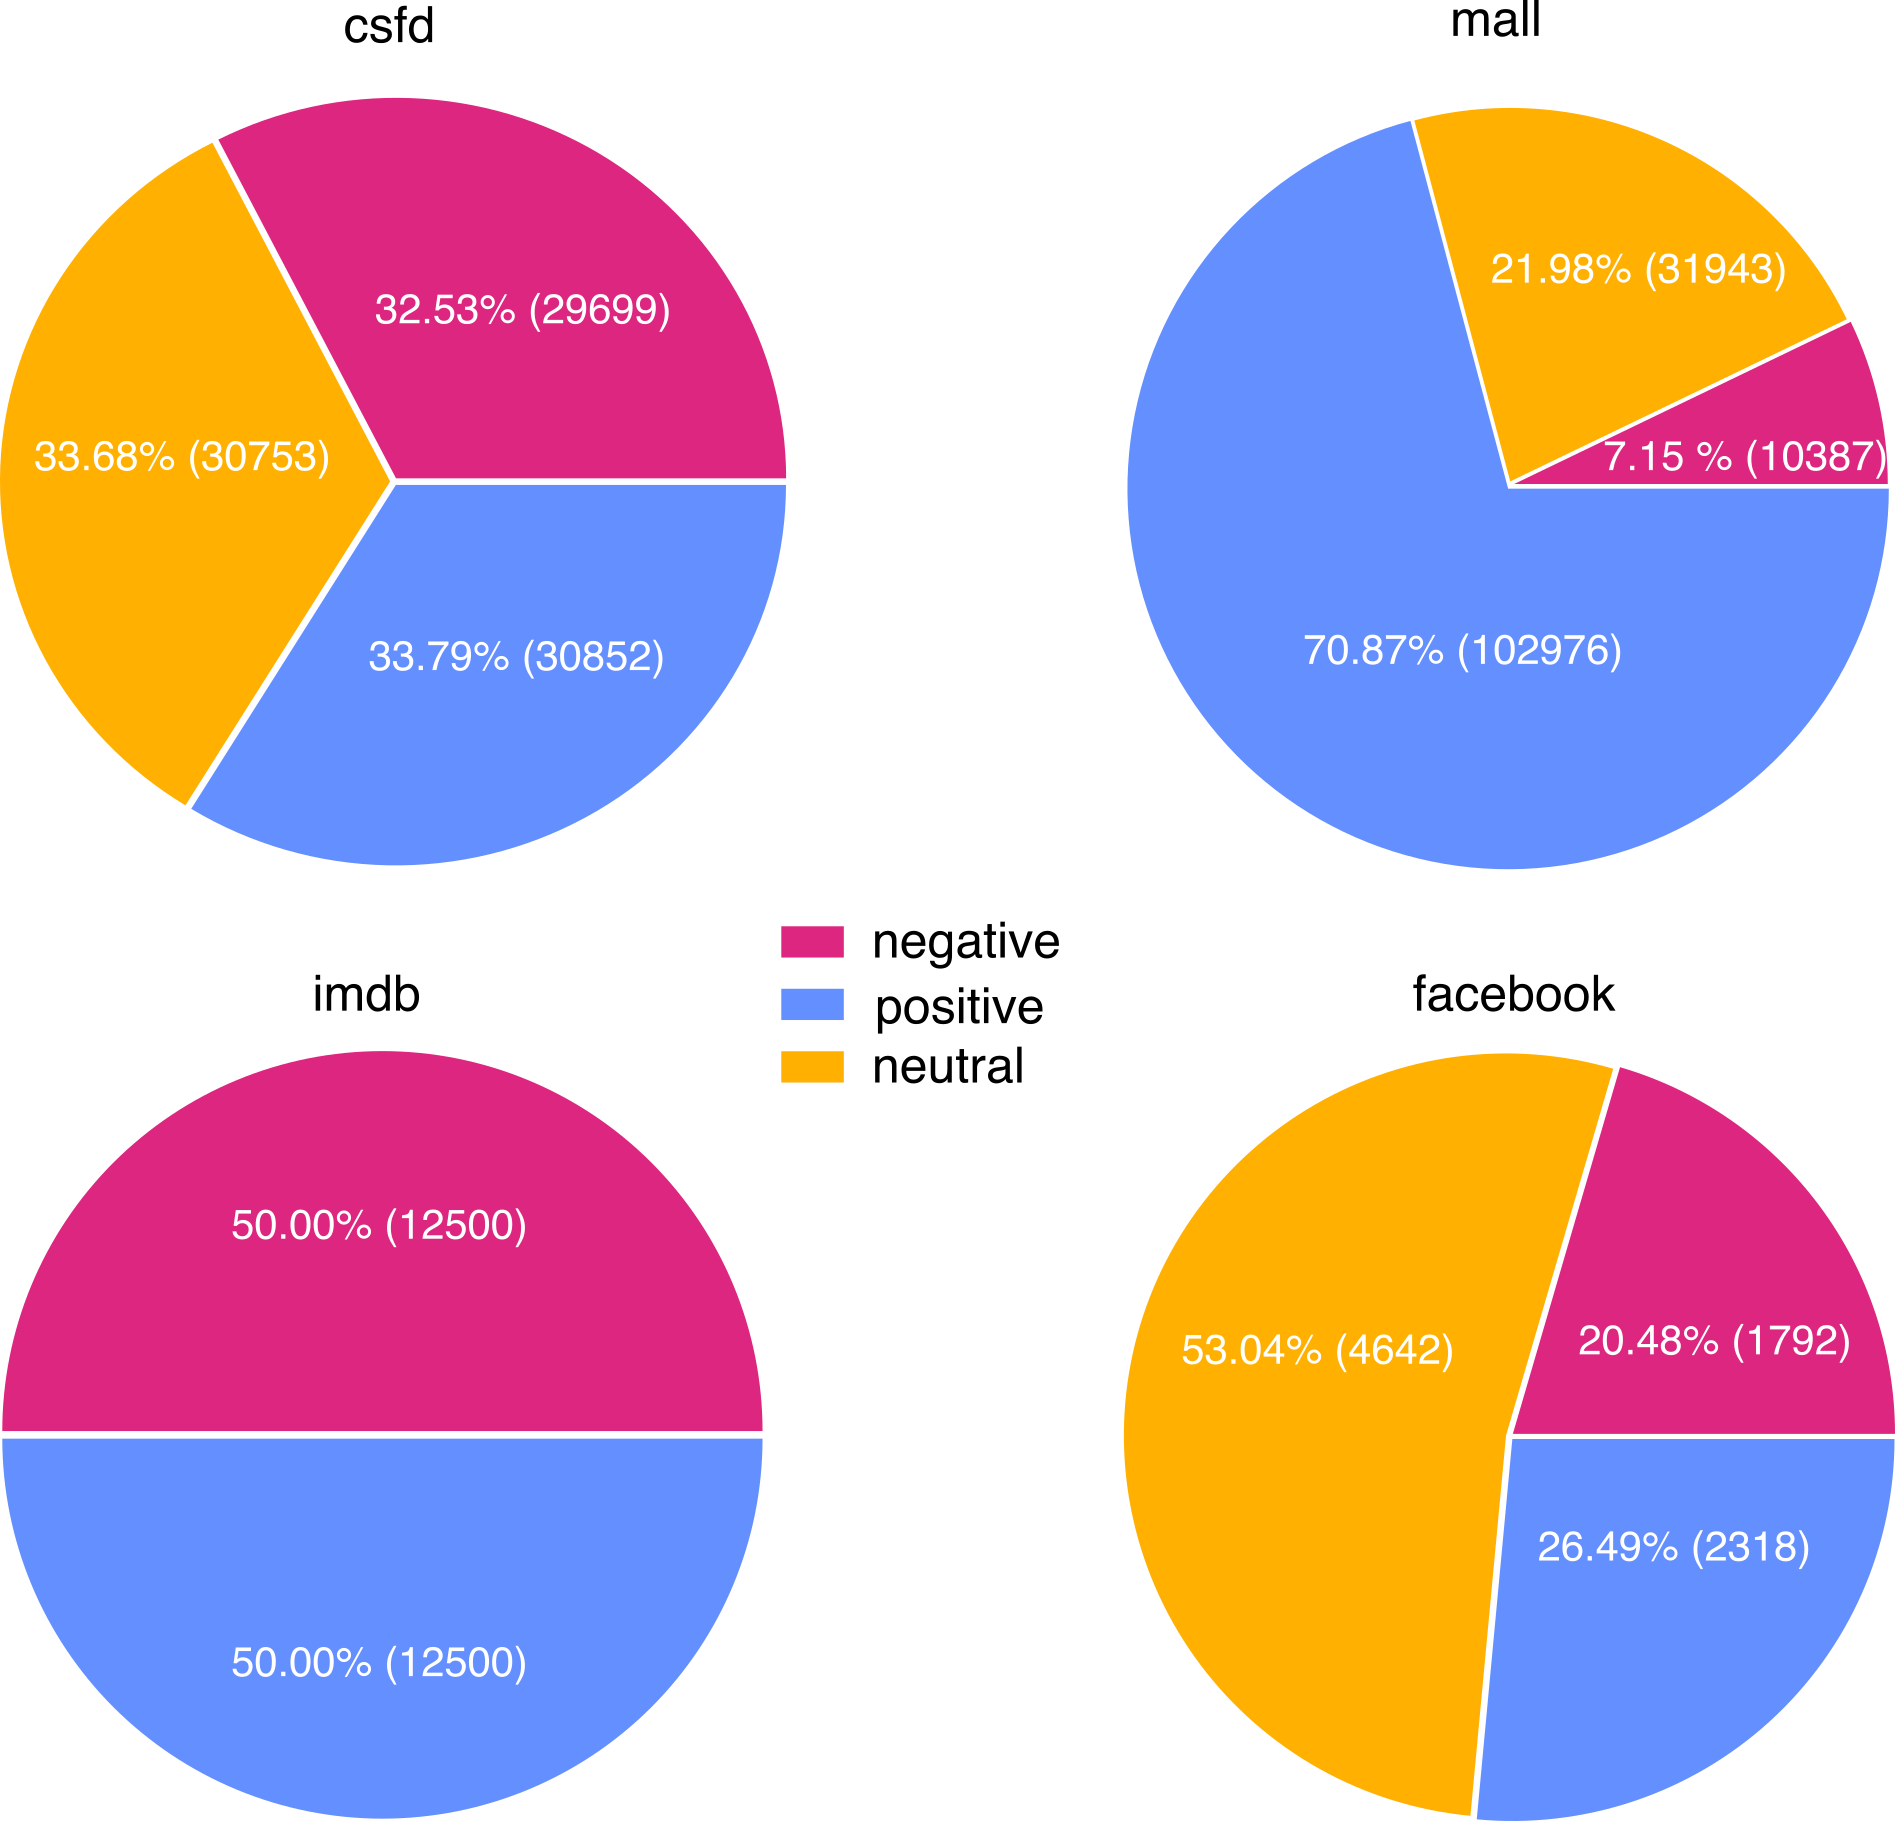
\includegraphics[width=1\columnwidth]{../img/dist_all.png}
\protect\caption{Distribution of positive/neutral/negative labels in each dataset.}
\label{pic:dist}
\end{figure}

%This was the the case for following experiments settings:
%learning rate of $2e-3$ for 10 epochs. This ended with predicting only one class (positive). Some progress showed the followign approach:"2:5e-5,1:2e-5, unfreezed" for facebook data only (which are balanced). This results are above 71 for accuracy (Test accuracy: 0.726
%F1 metrics: 0.7077061630227595 weighted).


\subsection{Experiments and Architecture}
The main division of experiments is by the input dataset -- each of Czech models separately and one joint dataset consisting of all Czech datasets, i.e. four different datasets. All variants performed both layers attention and an average of last four layers. As for the learning rate, all experiments were made with learning rate $3 \times 10^{-5}$ and there were always two types of learning rate decay -- cosine and inverse square root decay. 
\par
Network architecture is much simpler than in tagging and lemmatization task and corresponds to \textit{simple} setting of these tasks -- only BERT-like model and classification head consisting of layer with softmax activation function. %TODO a neni tam nahodou jeste neco?

%\begin{figure}[h]
%\centering
%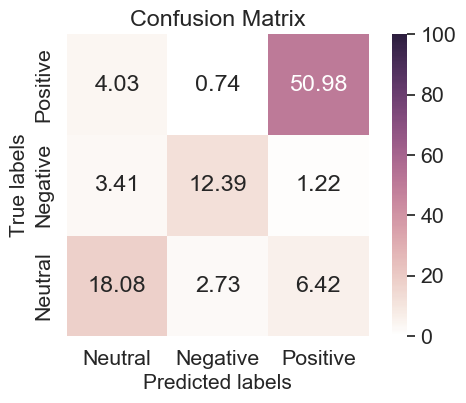
\includegraphics[width=1\columnwidth]{../img/confusion_matrix}
%\protect\caption{Normalized confusion matrix}
%\label{pic:conf1}
%\end{figure}

\subsection{Results and Discussion}

\begin{table}[!h]
\centering
  \begin{tabular}{|l||c|c|c||c|c|c|}
  \hline
    Model & Accuracy & F1 \\ \hline \hline
    baseline & 82.00 & 70.00  \\ \hline
    RobeCzech &  & 80.13 \\ \hline
    Czert & & 78.52 \\ \hline
    xlm-Roberta && 82.29 \\ \hline
    best(16) & 84.04 & 84.86 \\ \hline
  \end{tabular}
  \caption{ Baseline model (tf-idf) and the best model for all Czech data together.} %TODO popis } 
  \label{tab:res_czech}
\end{table}

\begin{table}[!h]
\centering
  \begin{tabular}{|l||c|c|c||c|c|c|}
  \hline
    Model & Accuracy & F1 \\ \hline \hline
    baseline & 69.07 & 69.00 \\ \hline
    best(43) & 81.50 & 81.37 \\ \hline
  \end{tabular}
  \caption{ Results for csfd dataset.} %TODO popis } 
  \label{tab:res_csfd}
\end{table}
\begin{table}[!h]
\centering
  \begin{tabular}{|l||c|c|c||c|c|c|}
  \hline
    Model & Accuracy & F1 \\ \hline \hline
    baseline & 84.72& 83.00 \\ \hline
    best(63) & 84.60 & 84.14 \\ \hline
  \end{tabular}
  \caption{Results for mall dataset.} %TODO popis } 
  \label{tab:res_mall}
\end{table}
\begin{table}[!h]
\centering
  \begin{tabular}{|l||c|c|c||c|c|c|}
  \hline
    Model & Accuracy & F1 \\ \hline \hline
    baseline & 67.30 & 63.00 \\ \hline
    best(45) & 81.80 & 81.65 \\ \hline
  \end{tabular}
  \caption{ Results for facebook dataset.} %TODO popis } 
  \label{tab:res_facebook}
\end{table}

%TODO crossvalidated \
%TODO tady mam best pro ruzne datasety a neni to uplne porovnatene

% Please add the following required packages to your document preamble:
% \usepackage{multirow}
\begin{table}[]
\centering
\resizebox*{!}{\textheight-2pt}{\begin{tabular}{|l|l|l|l||ll|}
\hline
\multicolumn{2}{|l|}{MODEL}       & EXPE                      & LRTYPE                & Acc    & F1   \\ \hline  \hline
1  & \multirow{6}{*}{mBERT}     & czech                     & \multirow{3}{*}{Isrd} & 0,81   & 0,81 \\ \cline{1-1} \cline{3-3} \cline{5-6} 
2  &                            & zero                      &                       & 0,50   & 0,45 \\ \cline{1-1} \cline{3-3} \cline{5-6} 
3  &                            & eng                       &                       & 0,81   & 0,81 \\ \cline{1-1} \cline{3-6} 
4  &                            & czech                     & \multirow{3}{*}{cos}  & 0,83   & 0,82 \\ \cline{1-1} \cline{3-3} \cline{5-6} 
5  &                            & zero                      &                       & 0,53   & 0,48 \\ \cline{1-1} \cline{3-3} \cline{5-6} 
6  &                            & eng                       &                       & 0,83   & 0,82 \\ \hline
13 & \multirow{4}{*}{RoBECzech} & czech                     & \multirow{2}{*}{isrd} & 0,81   & 0,81 \\ \cline{1-1} \cline{3-3} \cline{5-6} 
14 &                            & zero                      &                       & 0,55   & 0,48 \\ \cline{1-1} \cline{3-6} 
16 &                            & czech                     & \multirow{2}{*}{cos}  & 0,84   & 0,84 \\ \cline{1-1} \cline{3-3} \cline{5-6} 
17 &                            & zero                      &                       & 0,58   & 0,49 \\ \hline
19 & \multirow{6}{*}{mBERT}     & czech                     & \multirow{3}{*}{Isrd} & 0,82   & 0,81 \\ \cline{1-1} \cline{3-3} \cline{5-6} 
20 &                            & zero                      &                       & 0,54   & 0,48 \\ \cline{1-1} \cline{3-3} \cline{5-6} 
21 &                            & eng                       &                       & 0,82   & 0,81 \\ \cline{1-1} \cline{3-6} 
22 &                            & czech                     & \multirow{3}{*}{cos}  & 0,83   & 0,82 \\ \cline{1-1} \cline{3-3} \cline{5-6} 
23 &                            & zero                      &                       & 0,52   & 0,47 \\ \cline{1-1} \cline{3-3} \cline{5-6} 
24 &                            & eng                       &                       & 0,83   & 0,82 \\ \hline
31 & \multirow{4}{*}{RoBECzech} & czech                     & \multirow{2}{*}{isrd} & 0,83   & 0,83 \\ \cline{1-1} \cline{3-3} \cline{5-6} 
32 &                            & zero                      &                       & 0,58   & 0,50 \\ \cline{1-1} \cline{3-6} 
34 &                            & czech                     & \multirow{2}{*}{cos}  & 0,84   & 0,84 \\ \cline{1-1} \cline{3-3} \cline{5-6} 
35 &                            & zero                      &                       & 0,58   & 0,51 \\ \hline
37 & \multirow{2}{*}{mBERT}     & \multirow{7}{*}{facebook} & Isrd                  & 0,75   & 0,75 \\ \cline{1-1} \cline{4-6} 
38 &                            &                           & cos                   & 0,76   & 0,76 \\ \cline{1-2} \cline{4-6} 
41 & \multirow{5}{*}{RoBECzech} &                           & isrd                  & 0,80   & 0,80 \\ \cline{1-1} \cline{4-6} 
42 &                            &                           & simple                & 0,79   & 0,79 \\ \cline{1-1} \cline{4-6} 
43 &                            &                           & \multirow{3}{*}{cos}  & 0,82   & 0,81 \\ \cline{1-1} \cline{5-6} 
44 &                            &                           &                       & 0,81   & 0,81 \\ \cline{1-1} \cline{5-6} 
45 &                            &                           &                       & 0,82 & 0,82 \\ \hline
46 & \multirow{2}{*}{mBERT}     & \multirow{4}{*}{facebook} & Isrd                  & 0,76   & 0,76 \\ \cline{1-1} \cline{4-6} 
47 &                            &                           & cos                   & 0,77   & 0,77 \\ \cline{1-2} \cline{4-6} 
50 & \multirow{2}{*}{RoBECzech} &                           & isrd                  & 0,80   & 0,79 \\ \cline{1-1} \cline{4-6} 
51 &                            &                           & cos                   & 0,806  & 0,80 \\ \hline
52 & \multirow{2}{*}{mBERT}     & \multirow{8}{*}{mall}     & Isrd                  & 0,83   & 0,83 \\ \cline{1-1} \cline{4-6} 
53 &                            &                           & cos                   & 0,84   & 0,84 \\ \cline{1-2} \cline{4-6} 
56 & \multirow{2}{*}{RoBECzech} &                           & isrd                  & 0,83   & 0,83 \\ \cline{1-1} \cline{4-6} 
57 &                            &                           & cos                   & 0,85   & 0,84 \\ \cline{1-2} \cline{4-6} 
58 & \multirow{2}{*}{mBERT}     &                           & Isrd                  & 0,83   & 0,83 \\ \cline{1-1} \cline{4-6} 
59 &                            &                           & cos                   & 0,84   & 0,84 \\ \cline{1-2} \cline{4-6} 
62 & \multirow{2}{*}{RoBECzech} &                           & isrd                  & 0,84   & 0,84 \\ \cline{1-1} \cline{4-6} 
63 &                            &                           & cos                   & 0,85   & 0,84 \\ \hline
64 & \multirow{2}{*}{mBERT}     & \multirow{8}{*}{csfd}     & Isrd                  & 0,81   & 0,81 \\ \cline{1-1} \cline{4-6} 
65 &                            &                           & cos                   & 0,82   & 0,82 \\ \cline{1-2} \cline{4-6} 
68 & \multirow{2}{*}{RoBECzech} &                           & isrd                  & 0,83   & 0,83 \\ \cline{1-1} \cline{4-6} 
69 &                            &                           & cos                   & 0,85   & 0,85 \\ \cline{1-2} \cline{4-6} 
70 & \multirow{2}{*}{mBERT}     &                           & Isrd                  & 0,82   & 0,82 \\ \cline{1-1} \cline{4-6} 
71 &                            &                           & cos                   & 0,82   & 0,82 \\ \cline{1-2} \cline{4-6} 
74 & \multirow{2}{*}{RoBECzech} &                           & isrd                  & 0,83   & 0,83 \\ \cline{1-1} \cline{4-6} 
75 &                            &                           & cos                   & 0,84   & 0,84 \\ \hline
\end{tabular}}
\caption{This table presents complete results on the sentiment task. }
\label{tab:res_all_sent}
\end{table}



%Because BERT model was trained on multilingual data, it is naturally not so good in language minoritly presented in the Bert's training data. When transfering the learned knowledge to czech sentiment task, we actually want to improve model in two ways: teach it something more specific about given task, i.e., sentiment, and improve its knowledge about selected language (czech in this case). By using czech sentiment dataset, both thing are incorporated into training. To obtained better results and following the \citep{Putra}, I also selected english sentiment dataset. The idea behind is that BERT is quite good in english and maybe can learn faster useful knowledge about the given task from data in more familiar language.



%Baseline for this task is tf-idf method %TODO nekde je popsana v prni kapitole
%, which resulted in 
%[[ 4310   102  3015]
 %[  685  1016   779]
 %[  842    48 20227]]
 %             precision    recall  f1-score   support

%           0       0.74      0.58      0.65      7427
%           1       0.87      0.41      0.56      2480
 %          2       0.84      0.96      0.90     21117
%
%    accuracy                           0.82     31024
%   macro avg       0.82      0.65      0.70     31024
%weighted avg       0.82      0.82      0.81     31024




%results of zero2 without training
[[ 2809  6986   142]
 [ 1538  4621    53]
 [ 4787 15202   354]]
Test accuracy: 0.21330702619752273
F1 metrics: 0.1467527264529802

%jeste pusteno 35 to je s robeckem, jestli neni na tu cestinu prior lepsi

%TODO baseline u all neni macro ale weighted














